\subsection{Deltaspike}

\begin{frame}{Deltaspike}
\begin{itemize}
\item Framework che estende le funzionalità di CDI
\vspace{0.8em}
\item \textsl{Annotation-based}
\vspace{0.8em}
\item Gestisce i permessi degli utenti
\end{itemize}
\end{frame}

\begin{frame}{Architettura}
\begin{itemize}
\item Sicurezza su base metodo
	\begin{itemize}
	\item Classe \textsl{Authorizer}
	\vspace{0.8em}
	\item Annotare i metodi da controllare
	\end{itemize}
\vspace{0.8em}
\item Sicurezza su base pagina
	\begin{itemize}
	\item Gerarchia interfacce/classi -\textgreater  cartelle/pagine
	\vspace{0.8em}
	\item Classe \textsl{AccessDecisionVoter}
	\vspace{0.8em}
	\item Possibilità di specificare una pagina di errore con un messaggio adatto
	\end{itemize}
\end{itemize}

\end{frame}

\begin{frame}{Pagina di errore}
\centering
	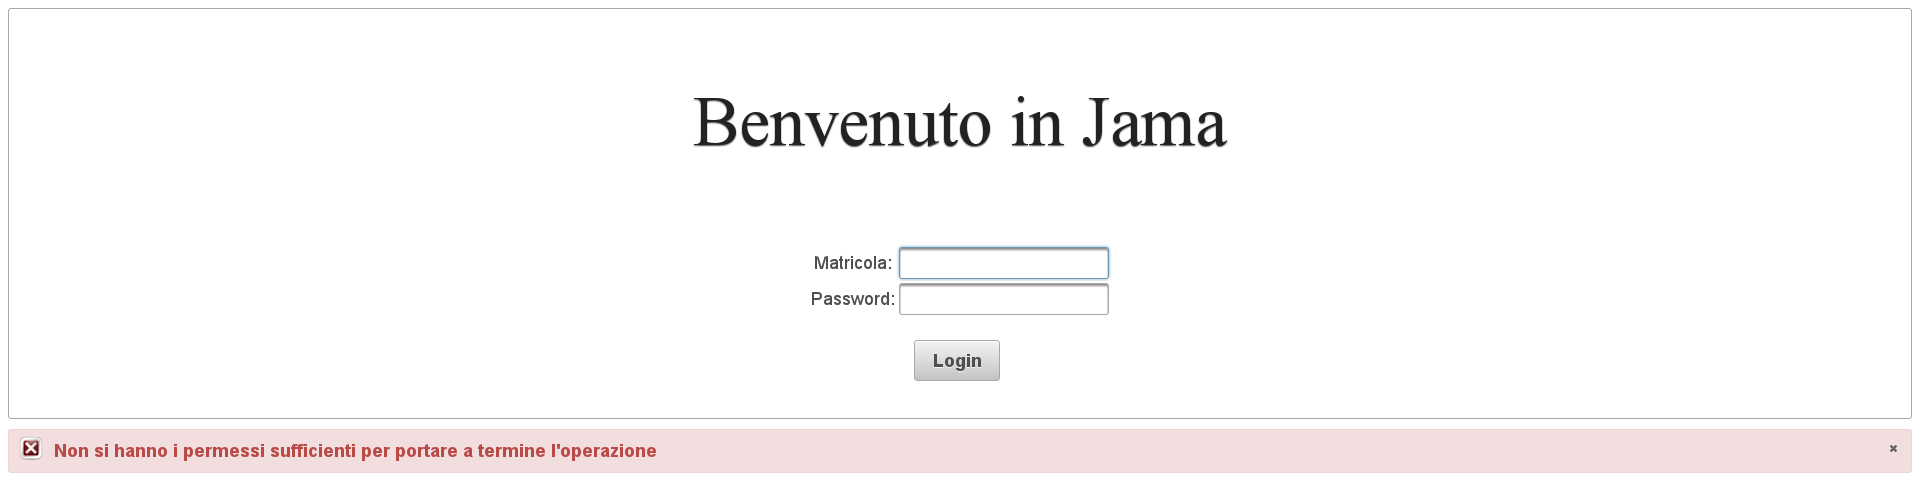
\includegraphics[width=1\textwidth]{PermessiInsufficienti.png}
\end{frame}

\section{Utenti}
\subsection{Modello}
\begin{frame}{Modello degli Utenti}
\begin{itemize}
\item Descrive la struttura delle classi riguardanti gli utenti ed i loro permessi
\end{itemize}	

\centering
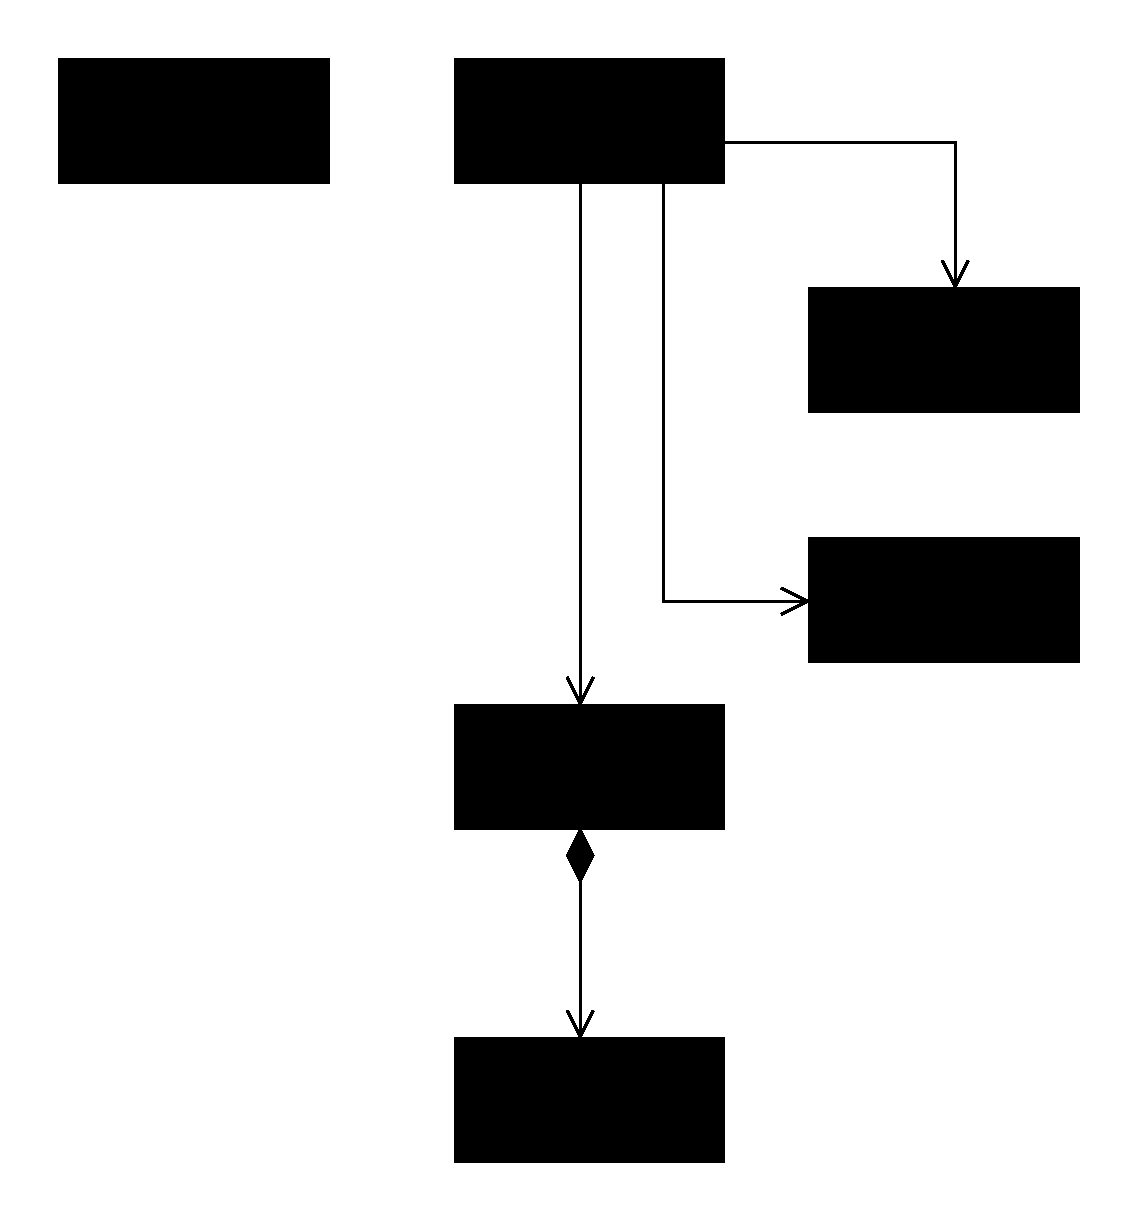
\includegraphics[width=0.4\textwidth]{user_model.eps}

\end{frame}

\subsection{Ruoli e Permessi}

\begin{frame}{Ruoli e Permessi}
\begin{itemize}
\item Admin
	\begin{itemize}
	\item Gestisce gli utenti ed i loro permessi
	\item Non afferisce a nessun dipartimento
	\end{itemize}
	
\vspace{0.8em}
\item Operator
	\begin{itemize}
	\item Gestisce le convenzioni del proprio dipartimento
	\end{itemize}

\vspace{0.8em}
\item Professor
	\begin{itemize}
	\item Visualizza le proprie convenzioni
	\item Allega documenti alle proprio convenzioni
	\end{itemize}

\vspace{0.8em}
\item Guest
	\begin{itemize}
	\item Nessun permesso
	\end{itemize}
\end{itemize}
\end{frame}

\section{Collaudo}
\subsection{Introduzione}
\begin{frame}{Collaudo}
\begin{itemize}
\item Il collaudo testa le funzionalità dell'applicazione, raggruppando insiemi di casi d'uso in scenari di alto livello da testare.
\vspace{0.8em}
\item Produce un documento che attesta la bontà dell'applicazione
\end{itemize}

\end{frame}

\begin{frame}{Scenari e Casi d'uso}

\begin{itemize}
\item Copertura dei casi d'uso
\end{itemize}

\begin{center}
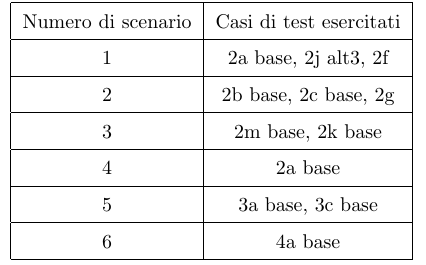
\includegraphics[width=0.5\textwidth]{collaudo.png}
\end{center}

\end{frame}

\subsection{Risultati}
\begin{frame}{Risultati}
\centering
\begin{figure}
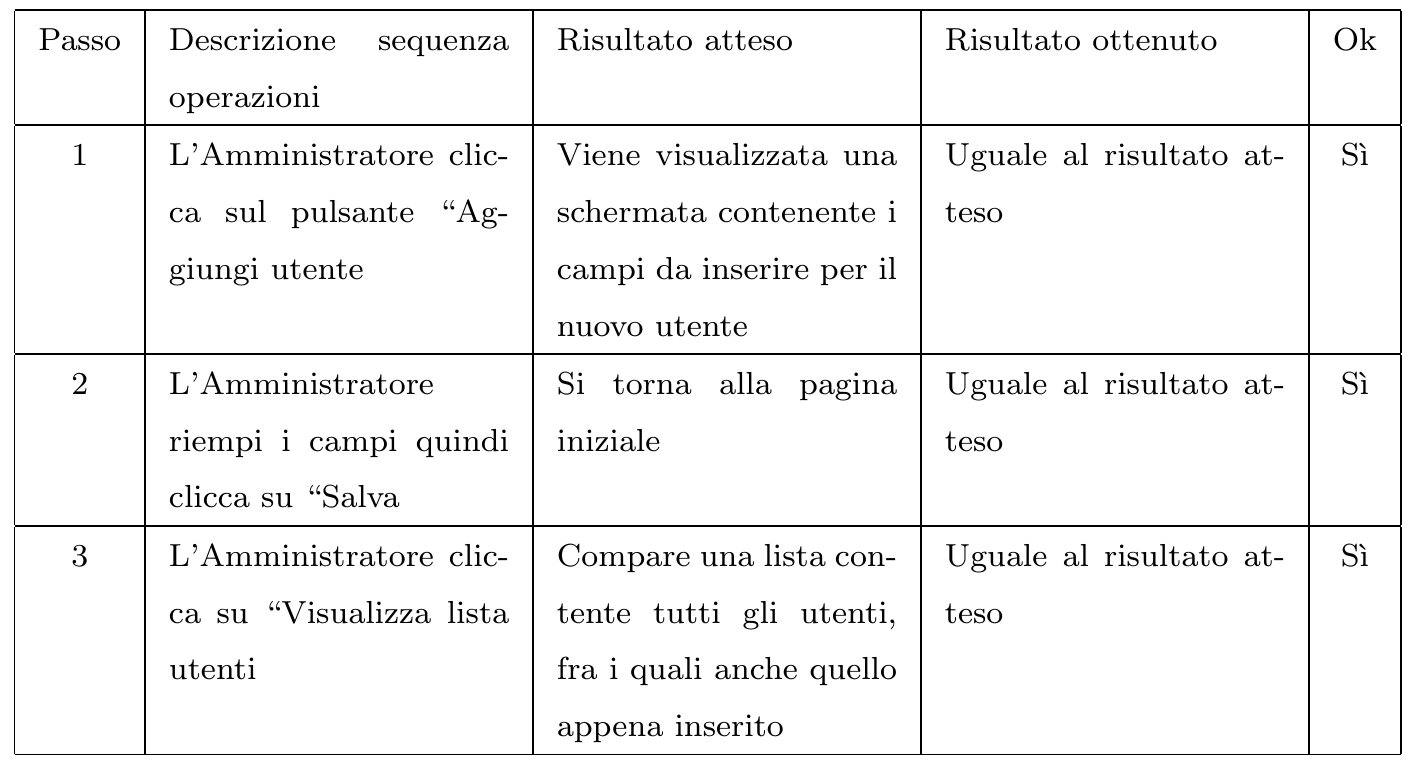
\includegraphics[width=1\textwidth]{scenario.png}
\caption{Scenario 6}
\end{figure}

\end{frame}

\section{Conclusioni}
\begin{frame}{Riassunto}
\begin{itemize}
\item Il lavoro degli autori è consistito nella progettazione e sviluppo di una Web Application
\vspace{0.8em}
\item L'applicazione verrà usata all'interno dei dipartimenti della facoltà di Ingegneria con una possibile estensione ad altre facoltà
\end{itemize}

\end{frame}
\begin{frame}{Requisiti}
\begin{itemize}
\item L'applicazione si occupa della gestione delle convenzioni e dei contributi. Consente di:
\vspace{0.8em}
	\begin{itemize}
	\item inserire convenzioni
	\item inserire rate per una convenzione
	\item visualizzare le convenzioni inserite
	\item aggiornare i dati di una convenzione
	\item notificare le scadenze
	\end{itemize}
\end{itemize}
\end{frame}

\begin{frame}{Conclusioni}
\begin{itemize}
\item Sono state usate le seguenti tecnologie
	\begin{itemize}
	\item JPA
	\item CDI
	\item JSF
	\item Deltaspike
\end{itemize}
\end{itemize}
\end{frame}